\documentclass{beamer}
\usepackage{graphicx}
\usetheme{AnnArbor}

\begin{document}
\section{Workshop on Qt}
\title{Programming with the Qt Framework}
\author{Saurabh Sood}

\begin{frame}
\titlepage
\end{frame}

\begin{frame}{Table Of Contents}
\tableofcontents
\end{frame}

\section{A bit of introduction}
\begin{frame}{What is a framework?}
\pause
\begin{itemize}
\item A collection of tools and libraries to make certain tasks easier? \pause
\begin{itemize}
\item Eg: A Dynamic Array, Hashtables etc (Collections)
\item Generic Algorithms to achieve a certain task
\end{itemize}
\end{itemize}
\end{frame}

\section{About Qt}
\begin{frame}{What is Qt?}\pause
\begin{itemize}
\item Pronounced as 'Cute' ;) \pause
\item It is a \textit{cross platform}, development framework
\item Original Language is C++ with bindings in many languages (Ruby, Python etc) \pause
\end{itemize}
\end{frame}

\section{Features}
\begin{frame}{Some features of Qt}
\begin{itemize}
\pause
\item Modular Design
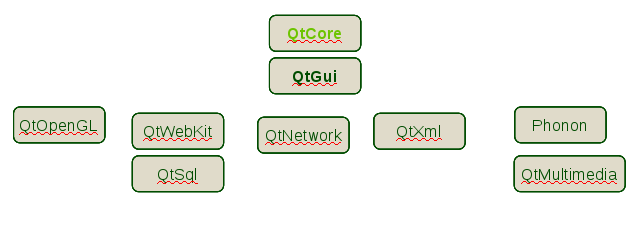
\includegraphics[width=10cm]{qt-mod.png}
\end{itemize}
\end{frame}

\begin{frame}{Macros and Introspection}
\pause
\begin{itemize}
\item Qt extends with \textit{macros} and \textit{introspection}
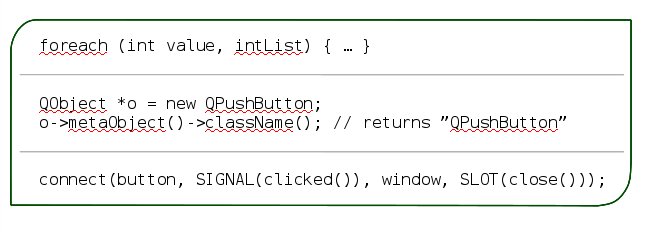
\includegraphics[width=10cm]{macros.png}
\end{itemize}
\end{frame}

\begin{frame}{Supported Platforms}
\pause
\begin{itemize}
\item *nix platforms
\item Windows
\item Android (through Necessitas)
\end{itemize}
\end{frame}

\begin{frame}{Applications using it...}
\pause
\begin{itemize}
\item KDE (The whole desktop environment along with the application suite)
\item VLC Media Player
\item Adobe Photoshop
\end{itemize}
\end{frame}

\section{Lets Dig in...}
\begin{frame}{Appease the Programming Gods...}
Hello World!!!
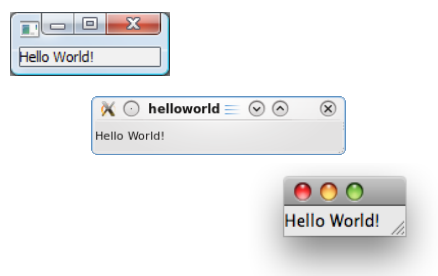
\includegraphics[width=10cm]{helloworld.png}
\end{frame}

\begin{frame}{Appease the Programming Gods...}
Hello World!!!
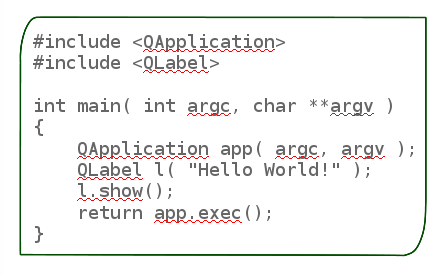
\includegraphics[width=10cm]{helloworld1.png}
\end{frame}

\begin{frame}
A Section by section disection of the code...
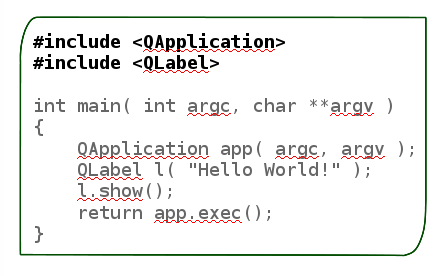
\includegraphics[width=10cm]{helloworld2.png}
\end{frame}

\begin{frame}
A Section by section disection of the code...
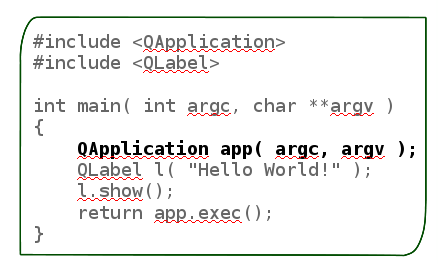
\includegraphics[width=10cm]{helloworld3.png}
\end{frame}

\begin{frame}
A Section by section disection of the code...
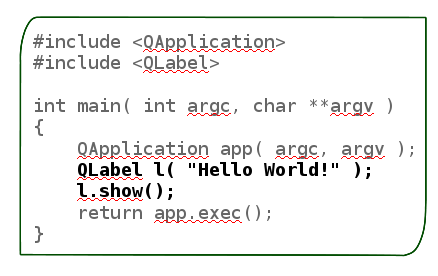
\includegraphics[width=10cm]{helloworld4.png}
\end{frame}


\begin{frame}
A Section by section disection of the code...
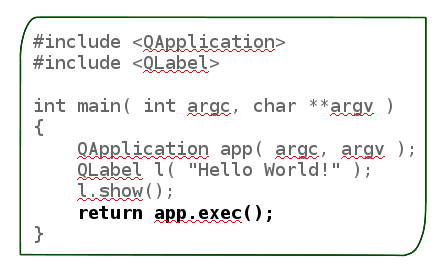
\includegraphics[width=10cm]{helloworld5.png}
\end{frame}

\section{Qt's event handling mechanism}
\begin{frame}{Signals and Slots}
\begin{itemize}
\pause
\item Passion \pause
\item Basic Programming skills though it may vary from project to project \pause
\item Soft Skills \pause
\item Long Term Commitment
\end{itemize}
\end{frame}

\begin{frame}{After GSoc?}
\pause
You are Awesomer!!!!
\end{frame}

\section{Becoming a mentor?}
\begin{frame}{Open Source communities cannot thrive without...}
\pause
mentors
\end{frame}

\begin{frame}{Who is a mentor?}
\pause
Anyone who is passing down his/her experience to new and existing community members
\end{frame}


\begin{frame}{You can become a mentor to}
\pause
\begin{itemize}
\item include new members into the project \pause
\item get some help to finish off a project for which you dont have the time \pause
\item share your knowledge \pause
\end{itemize}
\end{frame} 

\section{The Good, The Bad and The Ugly}
\begin{frame}{The Good}
\pause
\begin{itemize}
\item OBS Guys rock!!! \pause
\item Engagement with other projects \pause
\end{itemize}
\end{frame}


\section{The Bad}
\begin{frame}{The Bad}
\pause
\begin{itemize}
\item We do not have a list of ideas pouring in all the year \pause
\end{itemize}
\end{frame}

\section{The Ugly}
\begin{frame}{The Ugly}
\pause
\begin{itemize}
\item Too few mentors participating (Maybe we can solve it??) \pause
\end{itemize}
\end{frame}

\section{The Future}
\begin{frame}{The Future}
\pause
\begin{itemize}
\item Google Code-In
\item Google Summer of Code 2014
\end{itemize}
\end{frame}

\begin{frame}{Google Code-In}
\pause
\begin{itemize}
\item Targets school students
\item Different Goals
\pause
\begin{itemize}
\item Code
\item Documentation/Training
\item Outreach
\item QA
\item User Interface
\end{itemize}
\end{itemize}
\end{frame}

\section{Questions???}
\pause
\begin{frame}{Questions???}
\end{frame}

\end{document} 
